\section{Základní pojmy z planimetrie, rovinné útvary, úhly v nich}
\begin{definition}
  Nechť $A,B,C\in \mathbb E_2$ jsou tři body. Jestliže všechny tři leží (resp. neleží) na jedné přímce, řekneme, že jsou \textbf{kolineární} (resp. \textbf{nekolineární}).
\end{definition}

\begin{definition}
  Nechť $p,q\in \mathscr P$. Jestliže platí:
  \begin{enumerate}[$i.$]
    \item $p=q$, pak přímky $p,q$ se nazývají \textbf{splývající rovnoběžky},
    \item $p \ne q \land p\cap q = \emptyset$, pak přímky $p,q$ se nazývají \textbf{různé rovnoběžky},
    \item $p \ne q \land p\cap q \ne \emptyset$, pak přímky $p,q$ se nazývají \textbf{různoběžky}.
  \end{enumerate}
\end{definition}

\begin{definition}
  Nechť $p\in \mathscr P,A \in p, B \in p, A \ne B.$ Množinu
  \[
    P(A)=\left \{ X\in \mathbb E_2; X=B \lor X\,\mu\, AB \lor B\, \mu\, AX \right \}
  \]
  (resp. množinu $P(A)\cup \{A\}$) nazýváme \textbf{otevřenou} (resp. \textbf{uzavřenou}) \textbf{polopřímkou} $AB$ s počátkem v bodě $A$. Množinu
  \[
    Q(A)=\left \{ X\in \mathbb E_2; A\,\mu\, BX \right \}
  \]
  (resp. množinu $Q(A)\cup \{A\}$) nazýváme \textbf{otevřenou} (resp. \textbf{uzavřenou}) \textbf{polopřímku opačnou} k polopřímce $AB$ s počátkem $A$.
\end{definition}

\begin{definition}
  Nechť body $A,B\in \mathbb E_2, A\ne B$. Průnik uzanřených polopřímek $AB$ a $BA$ nazveme \textbf{úsečkou} $AB$. Body $A,B$ se nazývají \textbf{krajní body úsečky} $AB$, bod $X\,\mu \, AB$ se nazývá \textbf{vnitřní bod} úsečky $AB$.
\end{definition}

\begin{definition}
Nechť $a\in \mathscr P, A\notin a, B\notin a, A\ne B.$ Pak \textbf{přímka} $a$ \textbf{odděluje body} $A,B$ a zapisujeme $a\, \nu\, AB.$ V opčaném případě \textbf{přímka} $a$ \textbf{neodděluje body} $A,B$. Zapisujeme $a\, \overline \nu \,AB.$
\end{definition}

\begin{definition}
  Nechť $a \in \mathscr P$. Pak všechny $X\in \mathbb E_2 - a$ lze rozdělit do dvou podmnožin $P(a), Q(a)$ tak, že:
  \begin{enumerate}[$i.$]
    \item přímka $a$ odděluje každé dva body z různých podmnožin:
      \[
        \forall x \in P(a), \forall Y \in Q(a): a \, \nu \, XY
      \]
    \item přímka $a$ neodděluje žádné dva body z jedné podmnožiny
      \[
        \forall X, Y \in P(a) \land \forall X,Y \in Q(a): a \,\overline \nu\, XY.
      \]
  \end{enumerate}
  Pak množinu $P(a)$ (resp. množinu $Q(a)$) nazveme \textbf{otevřenou polorovinou s hraniční přímkou} $a$ (resp. \textbf{otevřenou polorovinou s hraniční přímkou} $a$ \textbf{opačnou k} $P(a)$). Množinu $P(a)\cup a$ (resp. $Q(a) \cup a$) nazveme \textbf{uzavřenou polorovinou s hraniční přímkou} $a$ (resp. \textbf{uzavřenou polorovinou s hraniční přímkou} $a$ \textbf{opačnou k} $P(a)$).
\end{definition}

\begin{definition}
  Nechť $A,B,V \in \mathbb E_2$ jsou tři různé nekolineární body. Průnik polorovin $VBA \cap VAB$ nazveme \textbf{konvexním úhlem} (zapisujeme $\sphericalangle BVA$), $V$ jeho \textbf{vrcholem}, polopřímky $VA, VB$ jeho \textbf{rameny}. \textbf{Nekonvexním úhlem} $BVA$ nazveme sjednocení polorovin opačných k polorovinám $VBA,VAB.$
\end{definition}

\begin{definition}
  Nechť $A,B,C\in \mathbb E_2$ jsou tři různé nekolineární body. \textbf{Trojúhelníkem} $ABC$ (značíme $\triangle ABC$) nazýváme \textbf{vrcholy} tohoto trojúhelníka, úsečky $AB, BC, CA$ jeho \textbf{stranami}.
\end{definition}

\begin{definition}
  Nechť $A,B\in \mathbb E_2.$ Přiřaďme uspořádané dvojici bodů $(A,B)$ reálné číslo označené $|AB|,$ pro něž platí:
  \begin{enumerate}[$i.$]
    \item $|AB|\geq 0,$ přičemž $|AB|=0 \iff A=B,$
    \item $|AB|=|BA|,$
    \item $C\, \mu \, AB \implies |AB|=|CB|+|AC|,$
    \item nechť $AB$ je polopřímka, $m\in \mathbb R^+_0.$ Pak $\exists ! C\in AB$ tak, že $|AC|=m.$
  \end{enumerate}
\end{definition}

\begin{definition}
  Každému konvexnímu úhlu $\sphericalangle AVC$ přiřaďme \textbf{velikost úhlu} (ozn. $|\sphericalangle AVC|$) ve stupních tak, že
  \begin{enumerate}[$i.$]
    \item nulový úhel má velikost $0^\circ$, přímý $180^\circ$,
    \item každý jiný konvexní úhel má velikost $n^\circ, $ kde $0^\circ< n ^\circ< 180^\circ, u \in \mathbb R,$
    \item jestliže polopřímka $VB$ prochází mezi rameny konvexního úhlu $\sphericalangle AVC$, pak $|\sphericalangle AVC|=|\sphericalangle AVB|+ |\sphericalangle BVC|$ a
    \item nechť $VA$ je polopřímka, $u \in \mathbb R, u \in \left < 0 ^\circ,180^\circ \right >$. Pak existuje polopřímka $VB$ taková, že $|\sphericalangle AVB|=u^\circ.$
  \end{enumerate}
\end{definition}

\begin{pozn}
  \textbf{Radián} je středový úhel příslušný v jednotkové kružnici kruhovému oblouku délky 1. Z definice plyne:
  \[
    360^\circ = 2\pi.
  \]
\end{pozn}

\begin{definition}
  Nechť $p,q\in \mathscr P$ jsou dvě různoběžky. Řekneme, že $p,q$ jsou na sebe \textbf{kolmé} (a zapisujeme $p\perp q$), jestliže všechny čtyři úhly, které spolu svírají, jsou shodné (a tedy pravé).
\end{definition}

\begin{pozn}[Klasifikace úhlů podle velikosti]
  Nechť $\alpha$ je velikost úhlu $|\sphericalangle ABC|$. Potom je úhel $|\sphericalangle ABC|$
  \begin{itemize}
    \item nulový, pokud $\alpha=0^\circ$,
  \item ostrý, pokud $0^\circ <\alpha < 90^\circ,$
  \item pravý, pokud $\alpha = 90^\circ,$
  \item tupý, pokud $90^\circ < \alpha < 180^\circ,$
  \item přímý, pokud $\alpha = 180^\circ,$
  \item konvexní, pokud $0^\circ \leq \alpha \leq 180^\circ,$
  \item nekonvexní, pokud $180^\circ < \alpha < 360^\circ$,
  \item plný, pokud $\alpha = 360^\circ,$
  \item kosý, pokud je ostrý nebo tupý.
  \end{itemize}
\end{pozn}

\begin{definition}
  Nechť $A,B\in \mathbb E_2$. \textbf{Vzdáleností bodů} $A,B$ nazveme délku úsečky $AB.$
\end{definition}


\begin{definition}
  Nechť $P\in \mathbb E_2, p \in \mathscr P.$ \textbf{Vzdáleností bodu} $P$ \textbf{od přímky} $p$ nazveme reálné číslo označené $\rho(P,p)$ takové, že $\rho(P,p)=|PP_0|,$ kde $P_0$ je kolmý průmět bodu $p$ na přímku $p$.
\end{definition}

\begin{definition}
  Nechť $a,b \in \mathscr P, a \parallel b.$ \textbf{Vzdáleností dvou přímek} $a,b$ nazveme reálné číslo označené $\rho(a,b)$ takové, že $\rho(a,b)=\rho(A,b),$ kde $A\in a$ je libovolný bod.
\end{definition}

\begin{definition}
  Nechť $a,b\in \mathscr P.$ \textbf{Odchylkou přímek} $a,b$ nazveme reálné číslo $\varphi^\circ\in \left <0, 180\right>$, kde $\varphi$ je velikost úhlu, který spolu přímky $a,b$ svírají. U rovnoběžek klademe $\varphi = 0^\circ.$
\end{definition}

\begin{definition}
  Dvojice úhlů:
  \begin{itemize}
    \item \textbf{vrcholové úhly} -- dvojice úhlů, jejichž ramena jsou opačné polopřímky
    \item \textbf{vedlejší úhly} --	dvojice úhlů, jejichž jedno rameno je společné a druhá ramena jsou opačné polopřímky
    \item \textbf{souhlasné úhly} -- dvojice úhlů, jejichž první ramena leží na jedné přímce a druhá ramena jsou rovnoběžná, přitom směr příslušných ramen je stejný
    \item \textbf{střídavé úhly}	-- dvojice úhlů, jejichž první ramena leží na jedné přímce a druhá ramena jsou rovnoběžná, přitom směr příslušných ramen je opačný
    \item \textbf{přilehlé úhly} -- dvojice úhlů, jejichž první ramena leží na jedné přímce a jdou do opačných směrů a druhá ramena jsou rovnoběžná
  \end{itemize}
\end{definition}

\begin{definition}
  Dvě polopřímky, ležící na téže přímce nazývámě \textbf{souhlasnými}, jestliže jedna z nich je podmnožinou druhé. V opačném případě je nazveme \textbf{nesouhlasnými}.
\end{definition}

\begin{definition}
  Nechť $\triangle ABC$. \textbf{Vnitřním úhlem} $\triangle ABC$ při vrcholu A (B, C) nazýváme $\sphericalangle CAB (ABC, BCA)$, \textbf{vnějším úhlem} $\triangle ABC$ při vrcholu A (B, C) pak vedlejší úhel k úhlu $\sphericalangle CAB (ABC, BCA)$.
\end{definition}

\begin{veta}
  Součet všech vnitřních úhlů v trojúhelníku je $180^\circ$.
\end{veta}

\begin{proof}
  \begin{figure}[h]
      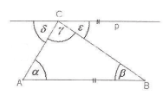
\includegraphics[width=\linewidth]{trojuhelnik_1.png}
  \end{figure}
\end{proof}

\begin{veta}
  Součet libovolných dvou vnitřních úhlů v trojúhelníku je menší něž $180^\circ$.
\end{veta}

\begin{proof}
  Plyne z předchozí věty a tvrzení, že vnitřní úhel v trojúhelníku je nenulový.
\end{proof}

\begin{veta}
  V každém trojúhelníku je velikost vnějšího úhlu při jednom vrcholu rovna součtu velikostí dvou zbylých vnitřních úhlů.
\end{veta}

\begin{proof}
  $$\alpha + \alpha^\prime = 180^\circ$$ (úhly vedlejší)
  $$\alpha + \beta + \gamma = 180^\circ$$
  $$\Rightarrow \alpha^\prime = \beta + \gamma$$
\end{proof}

\begin{definition}
  Trojúhelník se nazývá \textbf{rovnoramenný}, jestliže alespoň dvě jeho strany jsou shodné úsečky. Strany stejné délky nazveme \textbf{rameny}, tu třetí \textbf{základnou} a vrchol proti základně \textbf{vrcholem}.
  Trojúhelník se nazývá \textbf{rovnostranný}, jestliže všechny tři jeho strany jsou shodné úsečky.
  Trojúhelník se nazývá \textbf{pravoúhlý}, jestliže je jeden jeho vnitřní úhel pravý. Dvě strany, které jsou rameny pravého úhlu nazveme \textbf{odvěsnami}, tu třetí \textbf{přeponou}.
\end{definition}

\begin{definition}
  \textbf{Střední příčkou} trojúhelníku nazýváme úsečku spojující středy dvou stran trojúhelníka.
  \textbf{Těžnicí} trojúhelníku nazýváme úsečku spojující vrchol trojúhelníku se středem protější strany. Průsečík těžnic nazýváme \textbf{těžíště}.
  \textbf{Výškou} trojúhelníku nazýváme úsečku procházející vrcholem trojúhelníka, která je kolmá na přímku, na které leží protější strana trojúhelníku. Průsečík výšek nazýváme \textbf{ortocentrum}.
\end{definition}

\begin{veta}
  Každá střední příčka je rovnoběžná s protilehlou stranou a je dvakrát menší než protilehlá strana.
\end{veta}

\begin{proof}
  Trojúhelníky vrchol - střední příčka a vrchol - protilehlá strana jsou zjevně podobné s koeficientem 2.
\end{proof}

\begin{veta}
  Těžnice trojúhelníku se všechny protínají v jednom bodě, který je dělí v poměru $2:1$.
\end{veta}

\begin{proof}
  Doslova nevim, ve skriptách to není.
\end{proof}

\begin{veta}

\end{veta}
